\documentclass[11pt]{article}
\usepackage{hyperref} 
\usepackage{amsmath, amsfonts, amssymb}
\usepackage{graphicx}
\usepackage{float}
\usepackage[margin=1in]{geometry}
\usepackage{cancel}

\parindent0px

\emergencystretch=0pt
\pretolerance=150
\tolerance=10000
\hbadness=10000
\hfuzz=0pt

\title{Introduction to Linear Algebra Notes}
\author{Nathan Ueda}
\date{\today} 

\begin{document}
\maketitle 
\pagebreak
\tableofcontents 
\pagebreak

\section{Vectors and Matrices}
\subsection{Vectors and Linear Combinations}

\textbf{Vector Length:} For a vector $ v \in \mathbb{R}^n $, its length is:

\[ \|v\|= \sqrt{v_1^2 + \cdots + v_n^2} \]

In words, the length of a vector is the square root of the sum of the squared components. \\

Given two vectors in $\mathbb{R}^2\ v, w$ with their tail starting from the origin
\begin{itemize}
    \item If they lie on the same line, the vectors are \textit{linearly dependent}.
    \item If they do not lie on the same line, the vectors are \textit{linearly independent}.
\end{itemize}
Therefore, the combinations $ c\textbf{v} + d\textbf{w} $ fill the $x-y$ plane unless $v$ is in 
line with $w$. \\

To fill $m$-dimensional space, we need $m$ independent vectors, with each vector having $m$
components.

\subsection{Lengths and Angles from Dot Products}

\textbf{Dot Product:} For two vectors $v, w \in \mathbb{R}^n$, their dot product is:

\[ v \cdot w = v_1 w_1 + \cdots + v_n w_n \]

The dot product of two vectors tells us what amount of one vector goes in the direction of
another. It tells us how much these vectors are working together.

\begin{itemize}
    \item $ v \cdot w > 0 $: The vectors point in somewhat similar directions. In other
    words, the angle between the two vectors is less than 90 degrees.
    \item $ v \cdot w = 0 $: The vectors are perpendicular. In other words, the angle 
    between the two vectors is 90 degrees.
    \item $ v \cdot w < 0 $: The vectors point in somewhat opposing directions. In other
    words, the angle between the two vectors is greater than 90 degrees.
\end{itemize}

Dot Product Rules (for two vectors, v, w):
\begin{itemize}
    \item $ \boldsymbol{v} \cdot \boldsymbol{w} = w \cdot v $
    \item $ \boldsymbol{u} \cdot (\boldsymbol{v} + \boldsymbol{w}) = \boldsymbol{u} \cdot 
    \boldsymbol{v} + \boldsymbol{u} \cdot \boldsymbol{w} $
    \item $ (c\boldsymbol{v}) \cdot \boldsymbol{w} = c(\boldsymbol{v} \cdot \boldsymbol{w}) $
\end{itemize}

\textbf{Cosine Formula:} If $v$ and $w$ are nonzero vectors, then:
\[ \cos \theta = \frac{v \cdot w}{\|v\| \|w\|}\]

\textbf{Unit Vectors:} A vector is a unit vector if its length is 1. \\
For a vector $u \in \mathbb{R}^n$:

\[ \|u\| = 1\]

For any vector $v \in \mathbb{R}^n$, as long as $v \ne 0$, dividing $v$ by its length will
result in a unit vector. In other words:

\[ u = \frac{v}{\|v\|} \]

\textbf{Cauchy-Schwarz Inequality:} 
\[ | v \cdot w | \le \|v\|  \|w\| \]
In words, the absolute value of the dot product of two vectors is no greater than the product 
of their lengths. \\

\textbf{Triangle Inequality:} 
\[\|v + w\| \le \|v\| + \|w\|\]
In words, the length of any one side (in this case $\|v+w\|$) of a triangle is at most the sum
of the length of the other triangle sides.

\begin{figure}[H] 
	\centering 
	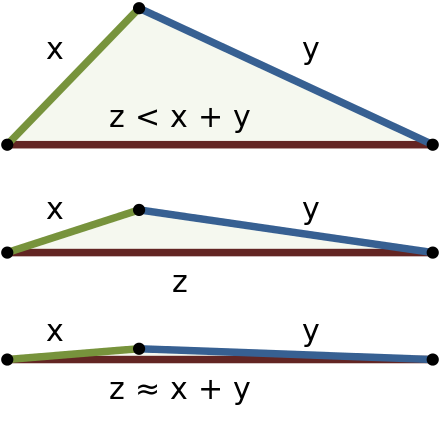
\includegraphics[width=2in]{imgs/triangle_inequality.png}
	\caption{This Squeeze Theorem}
\end{figure}

\subsection{Matrices and Their Column Spaces}

\textbf{Independence:} Columns are independent when each new column is a vector that we don't
already have as a combination of previous columns. The only combindation of columns that produces
$A\boldsymbol{x} = (0,0,0) $ is $ \boldsymbol{x} = (0, 0, 0) $. \\

\textbf{Column Space:} The column space, $\textbf{C}(A)$, contains all vectors 
$A\boldsymbol{x}$. In other words, it contains all combinations of the columns.

The \textbf{span} of the columns of $\boldsymbol{A}$ is the column space. \\

\textbf{Rank}: The number of independent columns of a matrix. This is equivalent to saying the
rank is the number of pivots in a matrix. \\

Rank Rules:
\begin{itemize}
    \item $ \text{rank}(A + B) \le \text{rank}(A) + \text{rank}(B) $
\end{itemize}

\subsection{Matrix Multiplication AB and CR}

To multiply two matrices $AB$, take the dot product of each row of $A$ with each column of $B$. \\ 
The number in row $i$, column $j$ of $AB$ is (row $i$ of $A$) $\cdot$ (column $j$ or $B$). \\

When $A \in \mathbb{R}^{m \times n}$ and $B \in \mathbb{R}^{n \times p}$:
\begin{itemize}
    \item  $AB \in \mathbb{R}^{m \times p}$
    \item $mp$ dot products are needed to carry out the matrix multiplication (one for each 
    entry in the matrix $AB$).
\end{itemize}

Matrix Multiplication Rules:
\begin{itemize}
    \item Associative: $(\boldsymbol{AB}) \boldsymbol{C}$
    \item Distributive: $\boldsymbol{A}(\boldsymbol{B} + \boldsymbol{C}) = \boldsymbol{AB} +
    \boldsymbol{BC}$
    \item Not Commutative: In general $\boldsymbol{AB} \ne \boldsymbol{BA}$
\end{itemize}

\section{Solving Linear Equations Ax = b}

\subsection{Elimination and Back Substitution}

For a matrix $A \in \mathbb{R}^{n \times n}$, there are three outcomes for 
$A\boldsymbol{x} = \boldsymbol{b}$:

\begin{enumerate}
    \item No solution
    \begin{itemize}
        \item $\boldsymbol{b}$ is not in the column space of $A$
        \item This occurs when the columns of $A$ are dependent and $\boldsymbol{b}$ is not in
        $C(A)$.
        \[\begin{bmatrix}
            2 & 4\\
            4 & 8
            \end{bmatrix} = \begin{bmatrix}
                16 \\
                \cancel{32}
                \end{bmatrix} \]
    \end{itemize}
    \item Exactly 1 solution
    \begin{itemize}
        \item $A$ has independent columns and an inverse matrix $A^{-1}$
    \end{itemize}
    \item Infinitely many solutions
    \begin{itemize}
        \item Columns of $A$ are dependent.
        \item This occurs when the columns of $A$ are dependent and $\boldsymbol{b}$ is in 
        $C(A)$
        \[\begin{bmatrix}
            2 & 4\\
            4 & 8
            \end{bmatrix} = \begin{bmatrix}
                16 \\
                32
                \end{bmatrix} \]
    \end{itemize}
\end{enumerate}

\textbf{Elimination:} A system that allows us to determine if $A\boldsymbol{x} = \boldsymbol{b}
$ has no solution, 1 solution, or infinitely many solutions. The goal of elimination is to
transform $A$ to an upper triangular matrix, $U$. \\ 

Elimination allows us to discover the number of pivots in $A \in \mathbb{R}^{n \times n}$ by 
creating $U$. If there are $n$ pivots in $U$, $U$ has full rank. This implies $A$ has exactly 
one solution. \\

\textbf{Back Substitution}:
If $U$ has full rank, back substituion allows us to find the solution. \\

\subsection{Elimination Matrices and Inverse Matrices}

\textbf{Elimination}

\begin{itemize}
    \item The basic elimination step subtracts a multiple of $\ell_{ij}$ of equation $j$ from
    equation $i$
\end{itemize}

\textbf{Inverse Matrices}

\begin{itemize}
    \item If $A$ is invertible, the one and only solution to $A\boldsymbol{x} = \boldsymbol{b}$
    is $\boldsymbol{x} = A^{-1}\boldsymbol{b}$
    \item Only square matrices can have inverses
    \item Invertible $\equiv$ non-singular $\equiv$ non-zero determinant $\equiv$ independent 
    columns
    \item Not invertible $\equiv$ singular $\equiv$ zero determinant $\equiv$ dependent columns
    \item If a matrix is invertible, the inverse is unique
    \item A triangular matrix has an inverse so long that it has no zero diagonal entries
\end{itemize}

\subsection{Matrix Computations and A = LU}

Elimination without row exchanges factors $A$ into $LU$. We can't find an $LU$ decomposition if 
row exchanges are needed during elimination. \\

\textbf{Gauss-Jordan elimination:}
\begin{itemize}
    \item An algorithm that allows us to determine if the inverse of a matrix exists, and if it
    does it exist, it allows us to determine what the inverse is. 
    \item Augment $A$ by $I$, that is $ \left[ A \ I \right]$, and through elementary row 
    operations, transform this matrix to $ \left[ I \ A^{-1} \right]$
\end{itemize}

\section{The Four Fundamental Subspaces}
\subsection{Vector Spaces and Subspaces}

To be a vector space means that all linear combinations $c\boldsymbol{v} + d\boldsymbol{w}$ of 
the vectors or matrices stay inside that space. \\

\textbf{Subspaces:} 
\begin{itemize}
    \item A subspace is a vector space entirely contained within another vector space
    \item All linear combinations of vectors in the subspace stay in the subspace
    \item Every subspace contains the zero vector
    \item Subspaces of $\mathbb{R}^3$:
    \begin{itemize}
        \item The single vector $(0,0,0)$
        \item Any line through $(0,0,0)$
        \item Any plane through $(0,0,0)$
        \item The whole space $\mathbb{R}^3$
    \end{itemize}
\end{itemize} 

\textbf{Column Space:}
\begin{itemize}
    \item The column space ($C(A)$) consists of all linear combinations of the columns
    \item To solve $A\boldsymbol{x} = \boldsymbol{b}$ is to express $\boldsymbol{b}$ as a
    combination of the columns
    \item The right side, $\boldsymbol{b}$, has to be in the column space produced by $A$, or 
    $A\boldsymbol{x} = \boldsymbol{b}$ has no solution
\end{itemize}

\textbf{Row Space:}
\begin{itemize}
    \item The row space of $A$ is the column space $C(A^T)$
    \item The rank of $A = \text{ rank of } A^T$
\end{itemize}

\textbf{Span:} 
\begin{itemize}
    \item The span of vectors $\boldsymbol{v}$ and $\boldsymbol{w}$ is the set of all of their 
    linear combinations.
    \item In other words, this tells us, given some set of vectors, which vectors are able to 
    be created by taking a linear combination of the vectors in the set. It is the vector  
    space we can reach (span) by taking linear combindations of the set of vectors.
    \item Independence is not required by the word span.
\end{itemize}


\end{document}